\clearpage
\section{Autenticazione e gestione profilo}

	\subsection{Registrazione}
		\label{registrazione}

		\begin{enumerate}

			\item Il primo passo per poter utilizzare l'applicazione \glossario{MaaP} è la registrazione. \`E possibile registrasi cliccando sul pulsante \texttt{Sign up} presente nella homepage (Figura \ref{fig:signUpButton}).

			\begin{figure}[H]
				\centering 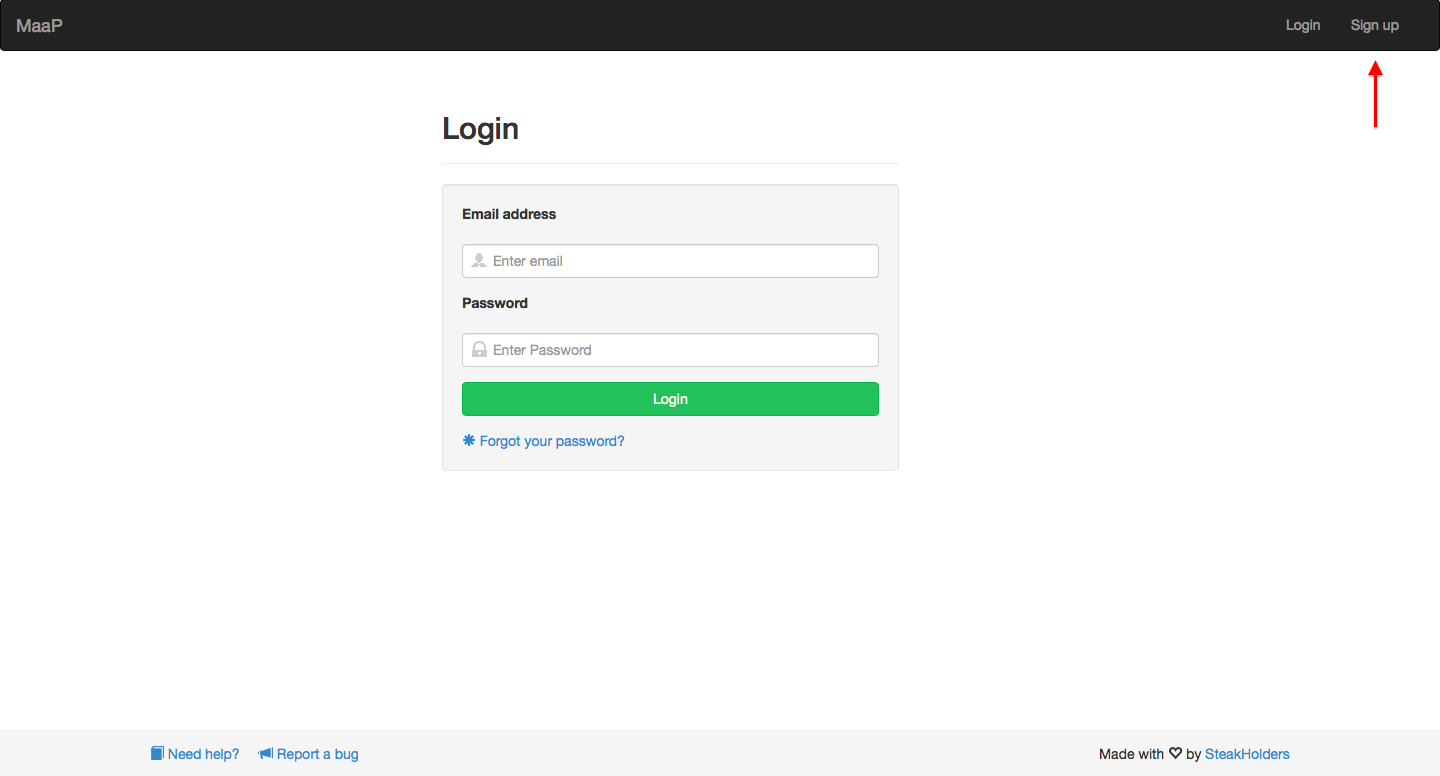
\includegraphics[width=1\textwidth]{img/pulsanteSignUp.png}
			\caption{ \label{fig:signUpButton} Pulsante per la registrazione}
			\end{figure}

			\item Verrà proposto un \glossario{form} (Figura \ref{fig:signUp}) da completare seguendo la procedura:
				\begin{itemize}
					\item \texttt{email}: inserire l'indirizzo mail con il quale registrarsi. Verrà utilizzato per il reset della password;
					\item \texttt{password}: inserire una password;
					\item \texttt{password confirmation}: inserire nuovamente la password del punto precedente;
					\item \texttt{Signup}: la pressione del tasto signup creerà il nuovo utente con le credenziali inserite.
				\end{itemize}


			\begin{figure}[H]
				\centering 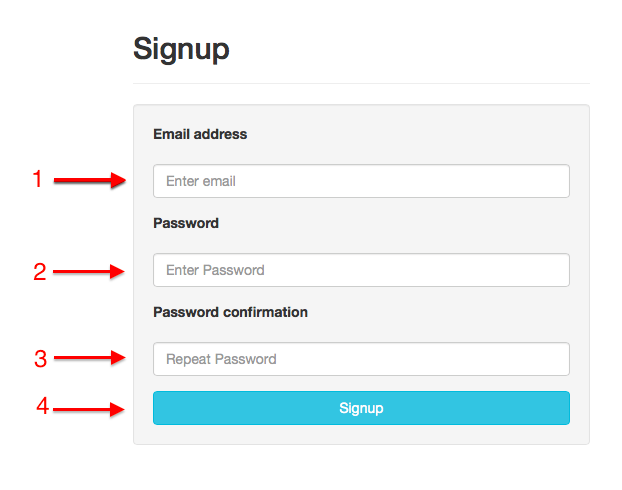
\includegraphics[width=0.6\textwidth]{img/signup.png}
			\caption{ \label{fig:signUp} Pagina di registrazione}
			\end{figure}

		\end{enumerate}

	\clearpage
	\subsection{Autenticazione}
		\label{autenticazione}

		\begin{enumerate}
			
			\item Per poter effettuare il login è necessario essere registrati (vedi \ref{registrazione}). \\
			Il login permette di accedere alla \glossario{dashboard} del sistema e quindi a tutte le funzionalità offerte da \glossario{MaaP}. Per autenticarsi è necessario compilare il \glossario{form} proposto nella pagina di login (Figura \ref{fig:loginButton}). 

			\begin{figure}[H]
				\centering 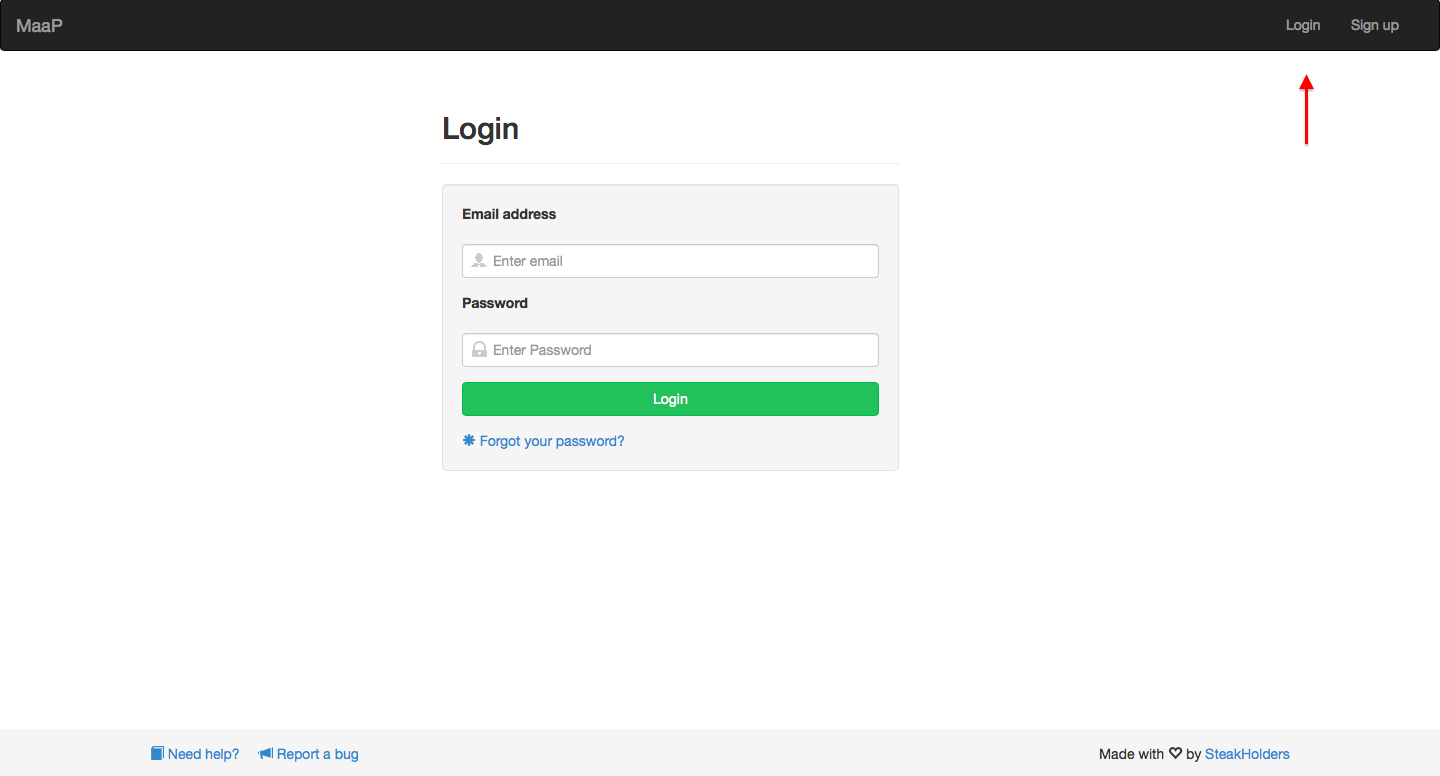
\includegraphics[width=1\textwidth]{img/pulsanteLogin.png}
			\caption{ \label{fig:loginButton} Pulsante per il login}
			\end{figure}

			\item Come illustrato in Figura \ref{fig:login}, viene richiesto di inserire \texttt{email} (1), \texttt{password} (2) e di cliccare sul pulsante \texttt{Sign in} (3). Terminata l'autenticazione, l'utente viene reindirizzato sulla \glossario{dashboard} (Figura \ref{visualizzazionedashboard}). Per il recupero password vedi \ref{recuperopassword}.

			\begin{figure}[H]
				\centering 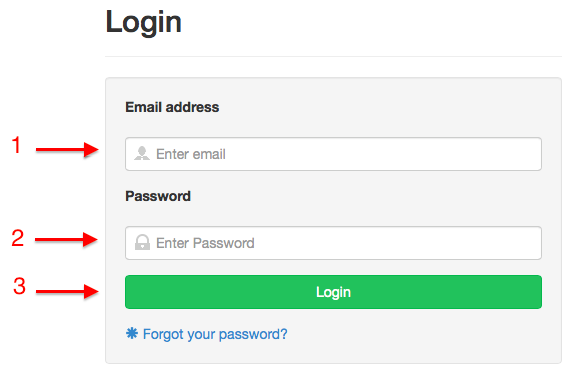
\includegraphics[width=0.6\textwidth]{img/login.png}
			\caption{ \label{fig:login} Pagina di login}
			\end{figure}

		\end{enumerate}

	\clearpage
	\subsection{Logout}
		\label{logout}

			Per poter effettuare il logout è necessario essere registrati (vedi \ref{registrazione}). \\
			Il logout permette di terminare la propria sessione di lavoro. Un volta effettuato il logout al successivo accesso alla piattaforma sarà richiesto di autenticarsi (vedi \ref{autenticazione}). Per effettuare il logout cliccare sul proprio indirizzo mail posto sulla barra del menù (Figura \ref{fig:logout}) e selezionare la voce \texttt{Logout}.

			\begin{figure}[H]
				\centering 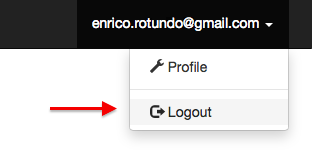
\includegraphics[width=0.5\textwidth]{img/logout.png}
			\caption{ \label{fig:logout} Pulsante per il logout}
			\end{figure}

	\clearpage
	\subsection{Recupero password}
		\label{recuperopassword}
		\begin{enumerate}

			\item Il recupero password avviene nel caso in cui l'utente abbia perso la password. Per poter procedere con un recupero password è necessario conoscere l'\texttt{email} di registrazione. Il recupero dalla password avviene partendo dalla pagina di login (Figura \ref{fig:loginButton}) cliccando sul link \texttt{Forgot your password?} (Figura \ref{fig:forgotpwd}).

			\begin{figure}[H]
				\centering 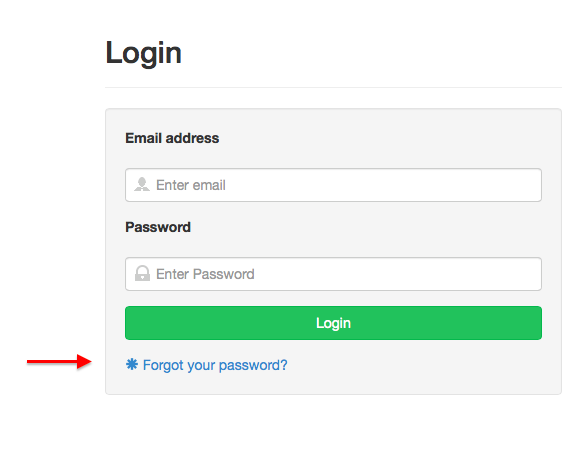
\includegraphics[width=0.6\textwidth]{img/forgotpwd.png}
			\caption{ \label{fig:forgotpwd} Pulsante per il recupero password}
			\end{figure}

			\item Verrà proposto un \glossario{form} (Figura \ref{fig:forgotPwdForm}) dove sarà richiesto di inserire l'\texttt{email di registrazione} (1) e cliccare il pulsante Submit per confermare l'operazione. (2).

			\begin{figure}[H]
				\centering 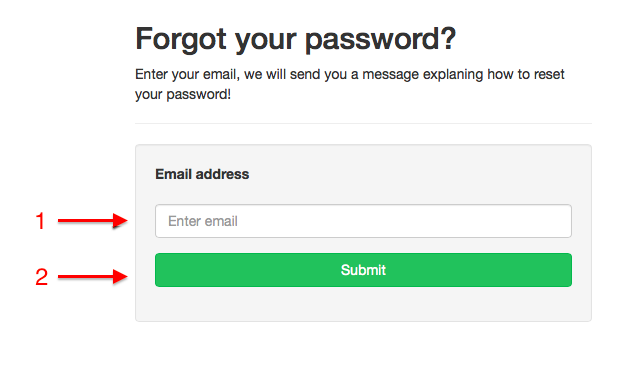
\includegraphics[width=0.6\textwidth]{img/forgotPwdForm.png}
			\caption{ \label{fig:forgotPwdForm} Form per il recupero password}
			\end{figure}

			\item L'utente riceverà un messaggio (Figura \ref{fig:mailResetPwd}) contenente l'url da seguire nella casella di posta associata all'indirizzo \texttt{email} inserito in fase di registrazione. 

			\begin{figure}[H]
				\centering 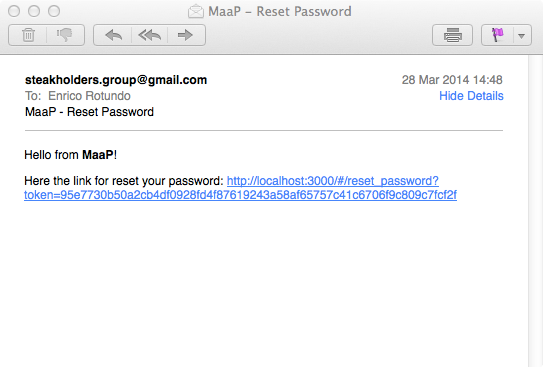
\includegraphics[width=0.8\textwidth]{img/mailResetPwd.png}
			\caption{ \label{fig:mailResetPwd} Email con link per reset password}
			\end{figure}

			\item Una volta raggiunto tramite \glossario{browser} il link ricevuto al punto precedente sarà necessario compilare il \glossario{form} (Figura \ref{fig:resetPwdForm}) per il reset della password inserendo la password due volte (1) e (2) e completando l'operazione con la pressione del pulsante \emph{Change Password} (3).

			\begin{figure}[H]
				\centering 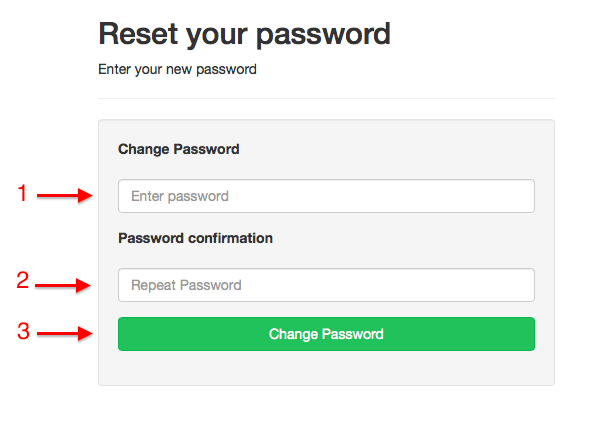
\includegraphics[width=0.6\textwidth]{img/resetPwdForm.png}
			\caption{ \label{fig:resetPwdForm} Form inserimento nuova password}
			\end{figure}

		\end{enumerate}

	\clearpage
	\subsection{Accesso e modifica profilo personale}
		\label{modificaprofilo}
		\begin{enumerate}

			\item Per accedere alla pagina di modifica del profilo cliccare sul proprio indirizzo mail posto sulla barra del menù (Figura \ref{fig:profileButton}) e selezionare la voce \texttt{Profile}.

			\begin{figure}[H]
				\centering 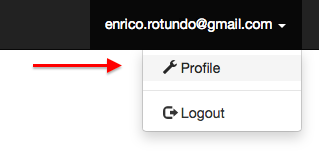
\includegraphics[width=0.5\textwidth]{img/profileButton.png}
			\caption{ \label{fig:profileButton} Pulsante pagina Profile}
			\end{figure}

			\item La pagina \emph{Profile} (Figura \ref{fig:showProfile}) visualizza le informazioni personali dell'utente (1), la modifica della password di registrazione avviene cliccando sul pulsante \emph{Edit password} (2).

			\begin{figure}[H]
				\centering 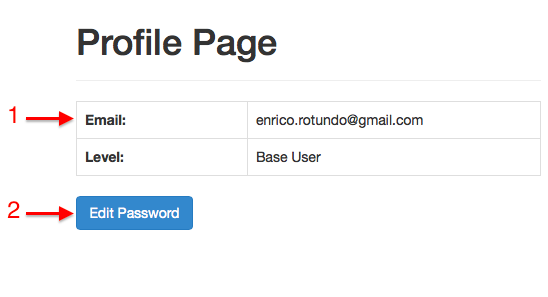
\includegraphics[width=0.8\textwidth]{img/showProfile.png}
			\caption{ \label{fig:showProfile} Pagina Profile}
			\end{figure}

			\item Viene proposto un form (Figura \ref{fig:changePwdForm}) nel quale va inserita la nuova password due volte (1) e (2), la password vecchia che si vuole sostituire (3) e confermare cliccando sul pulsante \emph{Save changes} (4). Se l'utente desidera interrompere l'operazione di modifica password può cliccare il pulsante \emph{Cancel}.

			\begin{figure}[H]
				\centering 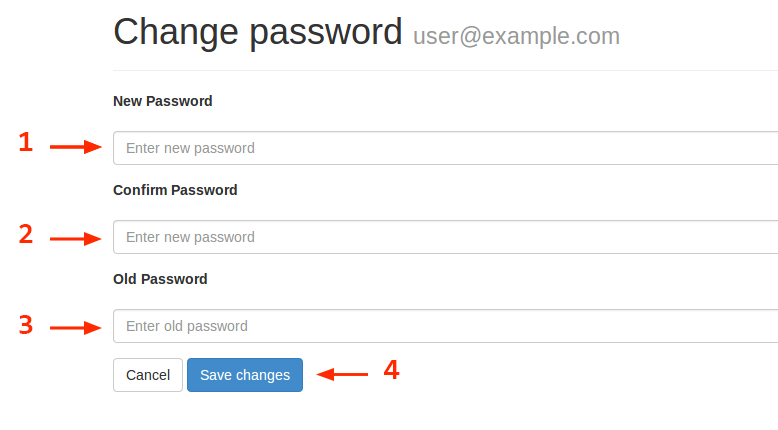
\includegraphics[width=0.9\textwidth]{img/changePwdForm.png}
			\caption{ \label{fig:changePwdForm} Form modifica password}
			\end{figure}

		\end{enumerate}
